\documentclass[12pt]{article}

 %%%%%%%%%% LOADING PACKAGES %%%%%%%%%% 
\usepackage{amsmath, amssymb, amsfonts, bm, mathtools} % math packages
\usepackage[table]{xcolor}
\usepackage{physics}
\usepackage{graphicx}
\usepackage{parskip}
\usepackage{fancyhdr}
\usepackage{vmargin}
\usepackage{tcolorbox}
\usepackage{url}
\usepackage[utf8x]{inputenc}
\usepackage{hyperref} % to click and go to pointed place in the document
\usepackage{cancel} % for easy cancellations
\usepackage{minted} % for highlighting code
\usepackage{comment} % for multi-line commenting

 %%%%%%%%%% SET DEFAULTS %%%%%%%%%% 
\newcommand{\smallspace}{\hspace{0.5cm}}
\setcounter{secnumdepth}{0} % for avoiding the numbering
\newenvironment{sfemph}{\begin{sffamily}\begin{emph}}{\end{sffamily}\end{emph}}
 % the text inside the exercise setup will be emphasized
 % Set defaults for minted
\setminted{frame=lines,
framesep=2mm,
baselinestretch=1.2,
bgcolor=,
fontsize=\footnotesize,
linenos
}

 %%%%%%%%%% INSERT YOUR DATA HERE %%%%%%%%%% 
\title{Market Analysis and Portfolio Optimization}						
\author{Federico Berto}			 				
\date{\today}											
\newcommand{\professor}{Woo Chang Kim}
\newcommand{\studentid}{20204817}
\newcommand{\coursename}{Introduction to Financial Engineering}
\newcommand{\courseid}{IE471}
\newcommand{\firstuniversityline}{Korea Advanced Institute of Science} % first line of university name
\newcommand{\seconduniversityline}{and Technology} % split the title for better compatibility. You may modify this part

 %%%%%%%%%% TITLE PAGE SETUP %%%%%%%%%% 
\setmarginsrb{3 cm}{2.5 cm}{3 cm}{2.5 cm}{1 cm}{1.5 cm}{1 cm}{1.5 cm}
\makeatletter
\let\thetitle\@title
\let\theauthor\@author
\let\thedate\@date
\makeatother
\pagestyle{fancy}
\fancyhf{}
\renewcommand{\headrulewidth}{0.4pt}
\rhead{\theauthor}
\lhead{AI Project 4}
\chead{\raisebox{-1ex}{
\includegraphics[width = 3cm]{images/university_secondary_logo.png}}}
\cfoot{Page \thepage}

 %%%%%%%%%% MAIN DOCUMENT %%%%%%%%%% 
\begin{document}

 %%%%%%%%%% TITLE PAGE SETUP %%%%%%%%%% 
\begin{titlepage}
	\centering
    \textsc{\LARGE  \firstuniversityline \\ \smallskip \seconduniversityline}\\[1 cm]	% university Name
    
\includegraphics[scale = 0.18]{images/university_main_logo.png}\\[1.5 cm]	% university Logo
    
	\textsc{\Large \coursename}\\[0.5 cm]
	\rule{\linewidth}{0.2 mm} \\[0.4 cm]
	{ \huge \bfseries {\thetitle}}\\
	\rule{\linewidth}{0.2 mm} \\[1.5 cm]
	
	\begin{minipage}{0.5\textwidth}
		\begin{flushleft} \large
			\emph{Professor:}\\
		    \professor \\ [0.5cm]
            \emph{Course ID:}\\
            \courseid
			\end{flushleft}
			\end{minipage}~
			\begin{minipage}{0.4\textwidth}
			\begin{flushright} \large
			\emph{Student:} \\
			\theauthor \\[0.5cm]
			\emph{ID number:}\\
			\studentid \\
		\end{flushright}
	\end{minipage}\\[2 cm]
	
\end{titlepage}

 %%%%%%%%%% TABLE OF CONTENTS %%%%%%%%%% 
%% Uncomment this part
% \tableofcontents
% \incl
% \pagebreak


 %%%%%%%%%% MAIN TEXT %%%%%%%%%% 
\section{Introduction}

The goal of this report is to describe the experimental process and result for analyzing the market and using prediction results for optimizing a portfolio. In particular, after predicting the future time-series of stock prices, we will optimize the weigthings for obtaining an optimal portfolio.\\
Let us briefly introduce the AI models we will use in the code.

\subsection{Recurrent Neural Networks}
\label{sec:rnn}
Recurrent Neural Networks (RNN) \cite{zaremba2014recurrent} are capable of dealing with sequences of data. As Figure \ref{fig:rnn} \footnote{Source: \href{https://kvitajakub.github.io/2016/04/14/rnn-diagrams/}{Github}}  shows, they form an unrolled, sequential undirected graph in which input data are fed sequentially.
\begin{figure}[h!]
    \centering
    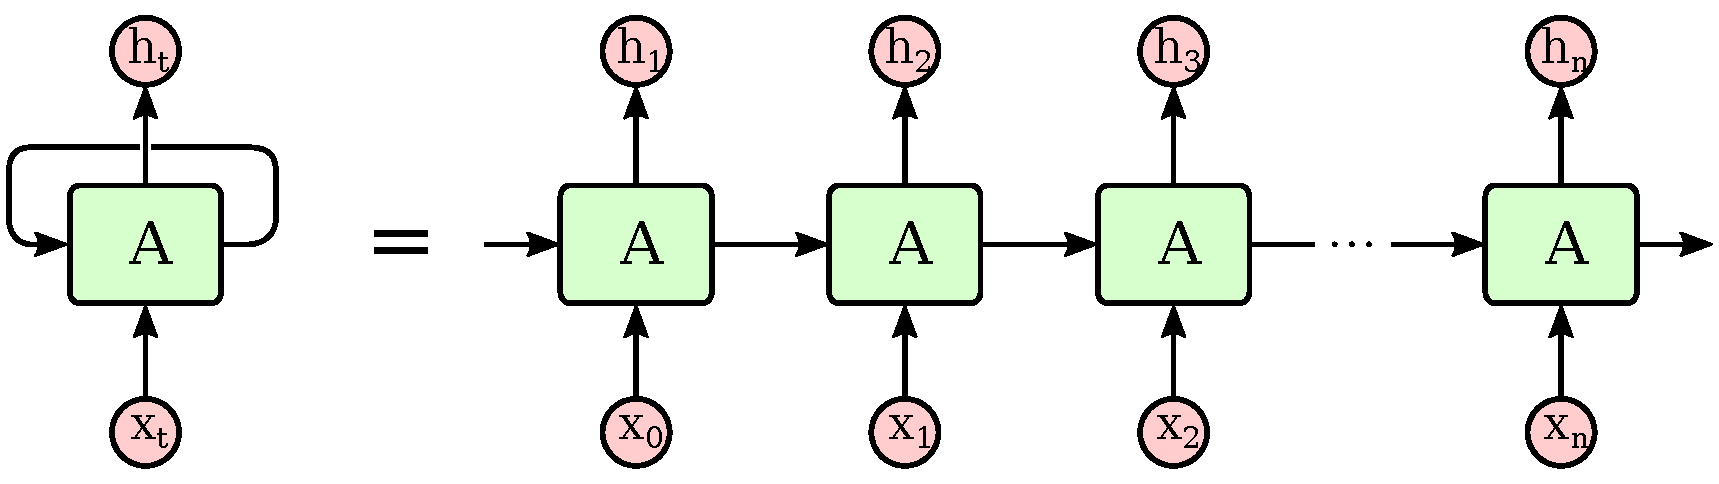
\includegraphics[width=0.7\linewidth]{images/rnn.pdf}
    \caption{Recurrent Neural Network (RNN) base model}
    \label{fig:rnn}
\end{figure}
The vanilla implementation's most notable problem is the so-called \textit{vanishing gradients} problem, in which long time series cannot be dealt with due the parameter updates using gradients; due to the sequential nature of RNNs, the further inputs in the time series are subject to more activation functions, causing updates to be almost independent from them.\\
For this reason, more advanced versions of Recurrent Neural Networks i.e GRU and LSTM have been created. Nonetheless, the simplicity of RNNs makes them suitable for shorter and less complex time series, since they are faster and also less prone to overfitting due to less parameters.

\subsection{Gated Recurrent Units}
\label{sec:gru}
Gated Recurrent Units (GRU) \cite{cho2014learning} were proposed as an RNN variant in 2014: they are similar to LSTMs without an output gate and has fewer parameters. Figure \ref{fig:gru} \footnote{Source: \href{https://en.wikipedia.org/wiki/Gated_recurrent_unit}{Wikimedia}} shows an overview of the architecture.
\begin{figure}[h!]
    \centering
    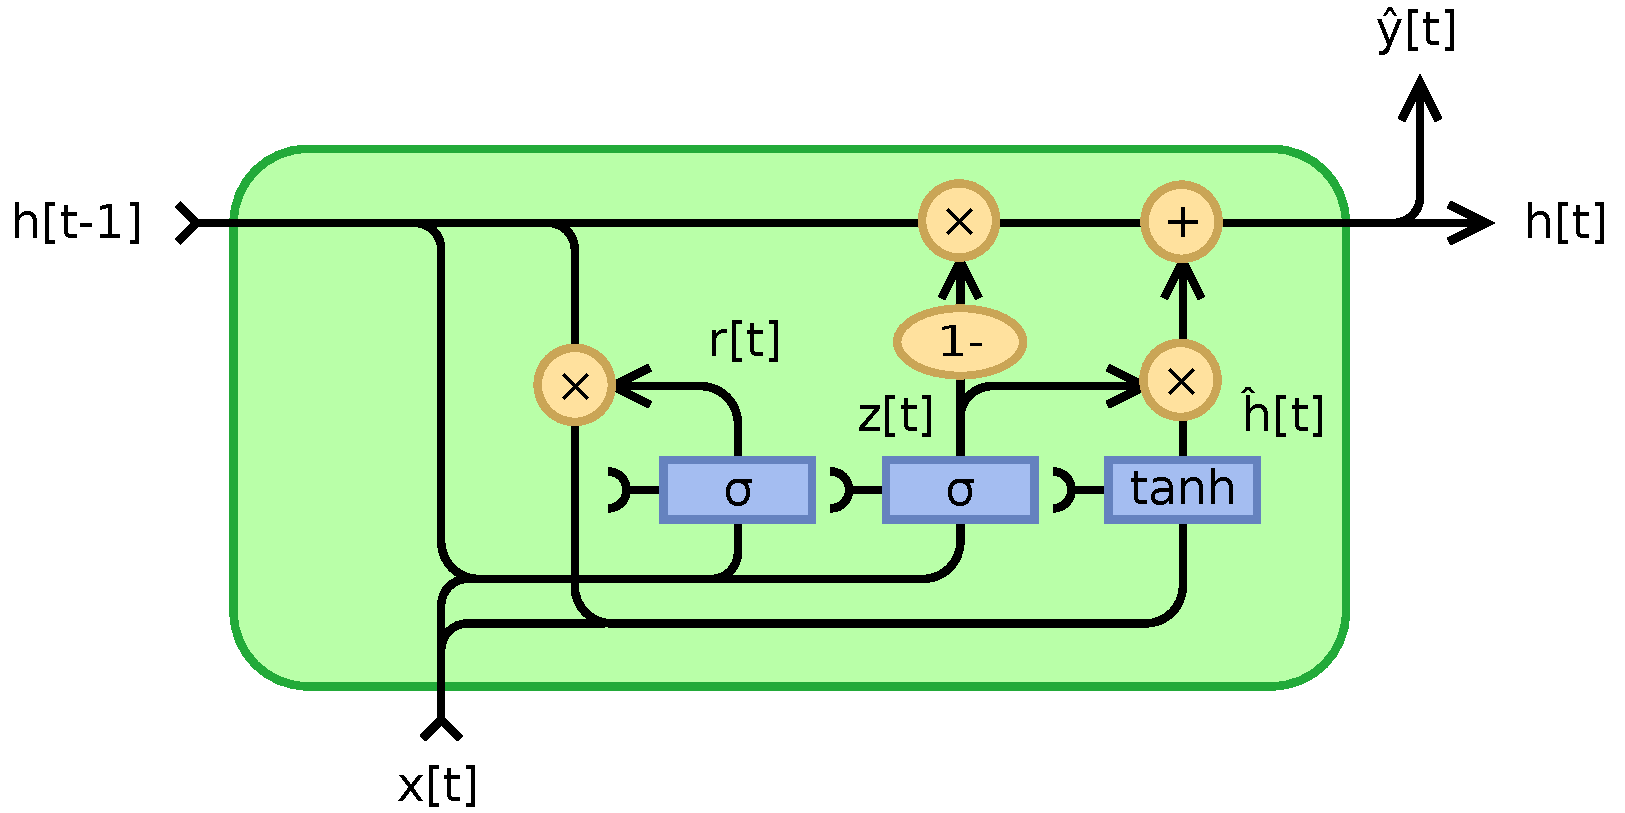
\includegraphics[width=0.7\linewidth]{images/Gated_Recurrent_Unit,_base_type.pdf}
    \caption{Gated Recurrent Unit (GRU) base model}
    \label{fig:gru}
\end{figure}
Having fewer parameters than LSTM \ref{sec:lstm}, GRUs have been shown to perform better on certain dataset and have better generalization capabilities with fewer data.

\subsection{Long Short-Term Memory}
\label{sec:lstm}
The prediction model is based on the Long Short-Term Memory (LSTM) \cite{hochreiter1997long} module in Figure \ref{fig:LSTM}\footnote{Source: \href{https://commons.wikimedia.org/wiki/File:LSTM_cell.svg}{Wikimedia}}, which is able to store past information of the data and is thus suitable for time series prediction.

\begin{figure}[h!]
    \centering
    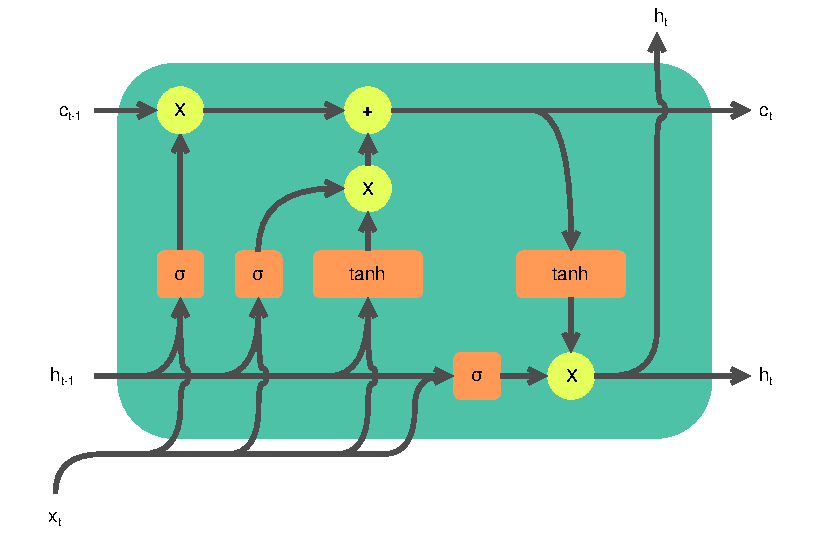
\includegraphics[width=0.7\textwidth]{images/LSTM_cell.pdf}
    \caption{LSTM cell}
    \label{fig:LSTM}
\end{figure}

Further details into the PyTorch \cite{pytorch} implementation can be found in the code, also available on the following \href{https://github.com/Juju-botu/financial-engineering-ai}{Github repository}.\footnote{Link: \href{https://github.com/Juju-botu/financial-engineering-ai}{\tt{https://github.com/Juju-botu/financial-engineering-ai}}.}

\section{Experiments}

\subsection{Portfolio Optimization on top US companies}
In this section we provide the required data for the report.

\paragraph{1.} Regimes analysis in Figures \ref{fig:gmm} and \ref{fig:markov}.

\begin{figure}[h!]
    \centering
    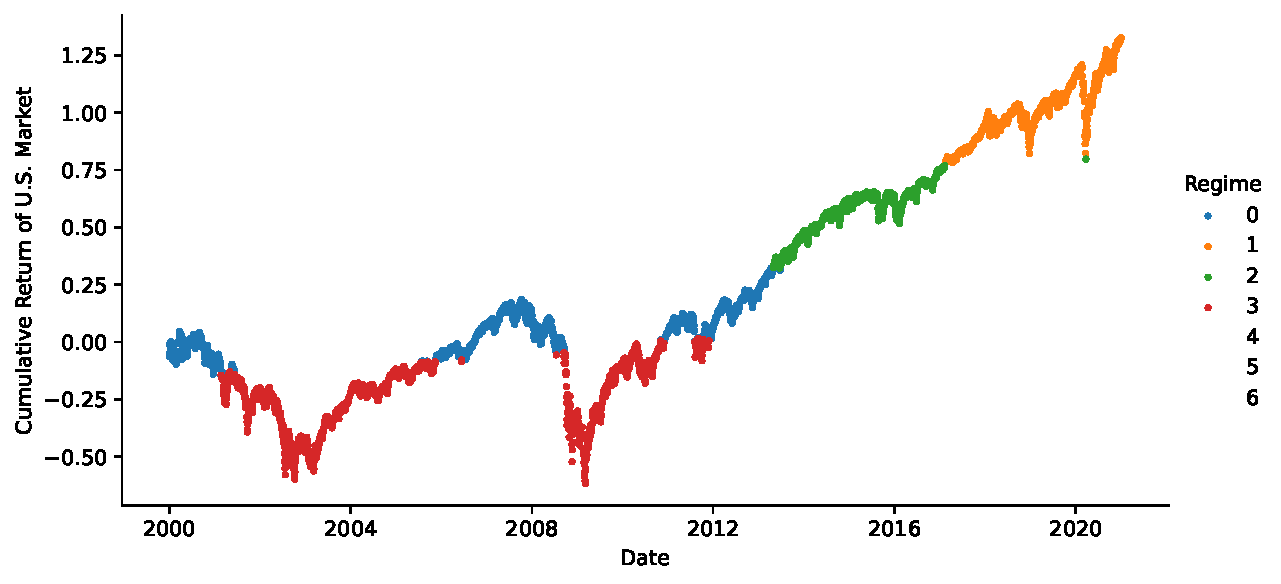
\includegraphics[width=0.9\textwidth]{images/market_gaussian.pdf}
    \caption{Market analysis with Gaussian Mixture Models}
    \label{fig:gmm}
\end{figure}


\begin{figure}[h!]
    \centering
    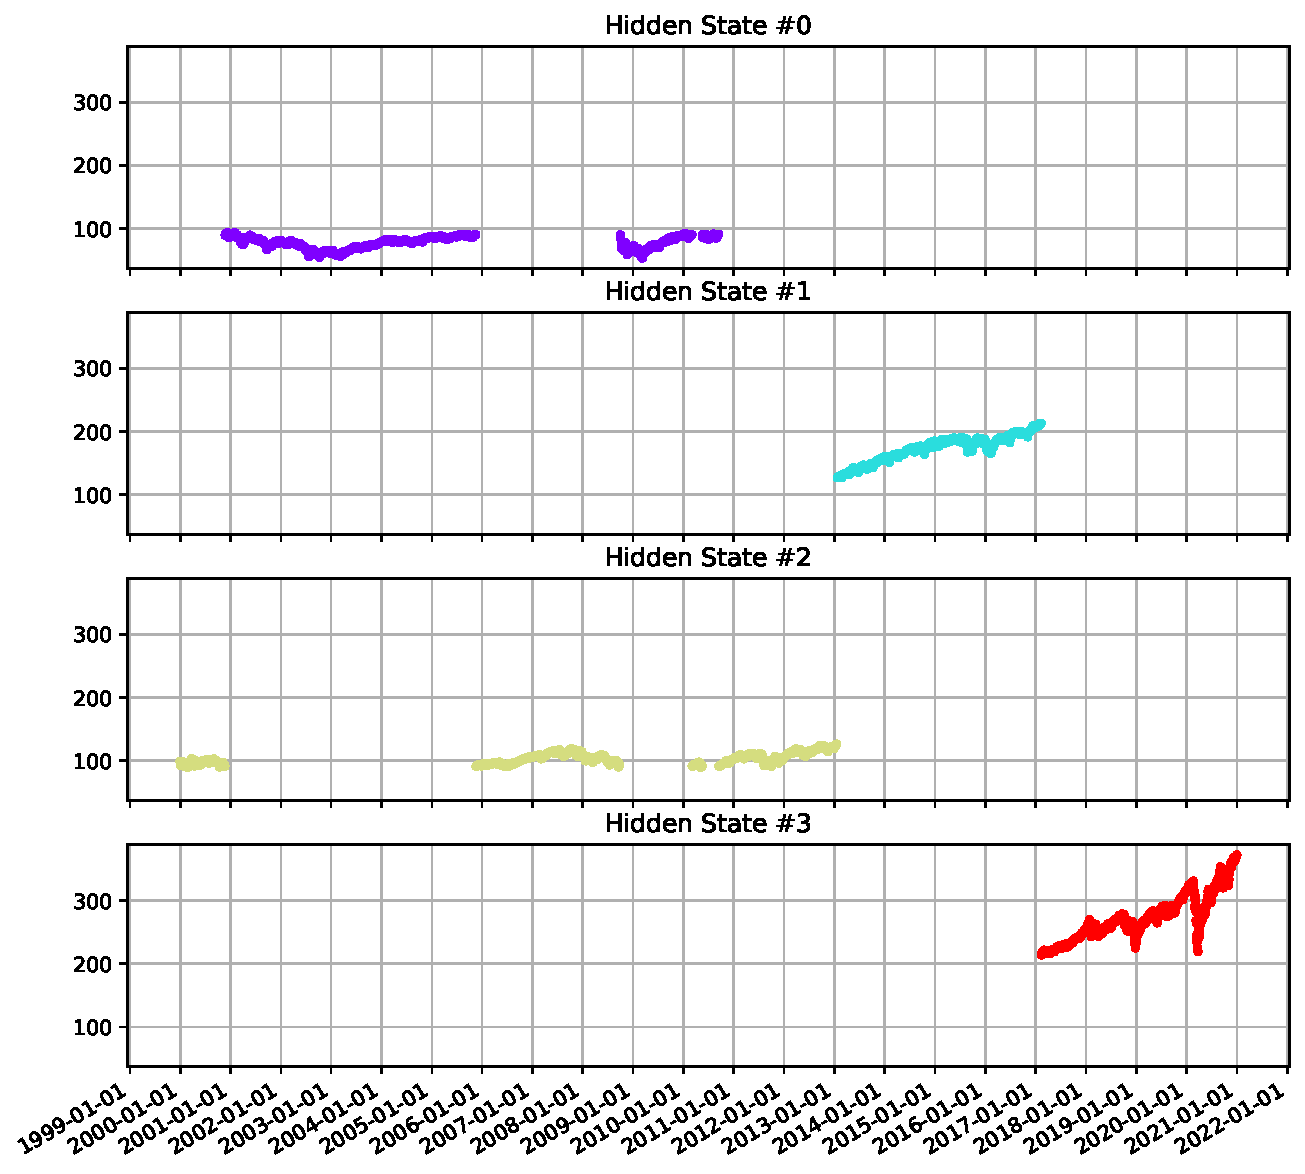
\includegraphics[width=0.9\textwidth]{images/hidden_markov.pdf}
    \caption{Market analysis with Hidden Markov Models}
    \label{fig:markov}
\end{figure}



\paragraph{2.} Mean values and covariance values of four regimes:

\begin{center}
\rowcolors{2}{gray!25}{white}     
    \begin{tabular}{l c c c c}
    \rowcolor{gray!50}
         &  \textbf{Regime 0}&  \textbf{Regime 1}&  \textbf{Regime 2}&  \textbf{Regime 3}\\
         \hline
         \text{Mean} & 137.5967 & 284.536 & 197.8587 & 106.826\\
         \text{Covariance} & 89.7873 & 1148.4455 & 298.8313 & 142.6559\\
    \end{tabular}
\end{center}

As we can see, Regime 3 is the one with lowest mean and indeed is the one corresponding to low cumulative returns, while Regime 1 corresponds with high cumulative returns and has high covariances.

\begin{itemize}
    \item Mean comparison: Regime 1 $>$ Regime 2 $>$ Regime 0 $>$ Regime 3
    \item Covariance comparison: Regime 1 $>$ Regime 2 $>$ Regime 3 $>$ Regime 0
\end{itemize}

\paragraph{3.} Losses for Netflix $\tt NFLX$ every 1000 epochs:

\begin{center}
\rowcolors{2}{gray!25}{white}     
    \begin{tabular}{l l}
    \rowcolor{gray!50}
        \bf{Epoch} & \bf{Loss} \\
        \hline
    0 & 0.3728 \\
    1000 &0.0003 \\
    2000 &0.0002 \\
    3000 &0.0001 \\
    4000 &0.0001 \\
    5000 &0.0001 \\
    6000 &0.0001 \\
    7000 &0.0001 \\
    8000 &0.0000 \\
    9000 &0.0000 \\
    10000 &0.0000 \\
    \end{tabular}
\end{center}

\paragraph{4.} $ \tt Results of Error Metrics (LSTM).csv$: attached to the zip file.

\paragraph{5.} Three portfolios’ last five cumulative returns:

\begin{center}
\rowcolors{2}{gray!25}{white}     
    \begin{tabular}{l c c c}
    \rowcolor{gray!70}
    \multicolumn{4}{c}{\textbf{Cumulative Returns of Portfolios}}\\
    \hline
    \rowcolor{gray!50}
        \bf{Date} & \bf{LSTM} & \bf{Equally Weighted}& \bf{Capitalization Weighted}\\
        \hline
        2020-12-24 00:00:00	&4.070533 &0.667722 &0.960323\\
        2020-12-28 00:00:00	&4.083723 &0.682366 &0.991312\\
        2020-12-29 00:00:00	&4.099815 &0.684749 &0.989239\\
        2020-12-30 00:00:00	&4.318745 &0.687135 &0.985936\\
        2020-12-31 00:00:00	&4.400515 &0.696872 &0.991695\\
    \end{tabular}
\end{center}

\paragraph{6.} Comparison of best porfolios: we can clearly see that in this case the LSTM portfolio outperformed both the Equally Weighted and the Capitalization Weighted portfolios; the final return was more than four times the cumulative return of the CPW portfolio.

\paragraph{7. } Portfolios performances in cumulative returns over time in Figure \ref{fig:portfolio_fin}:

\begin{figure}[h!]
    \centering
    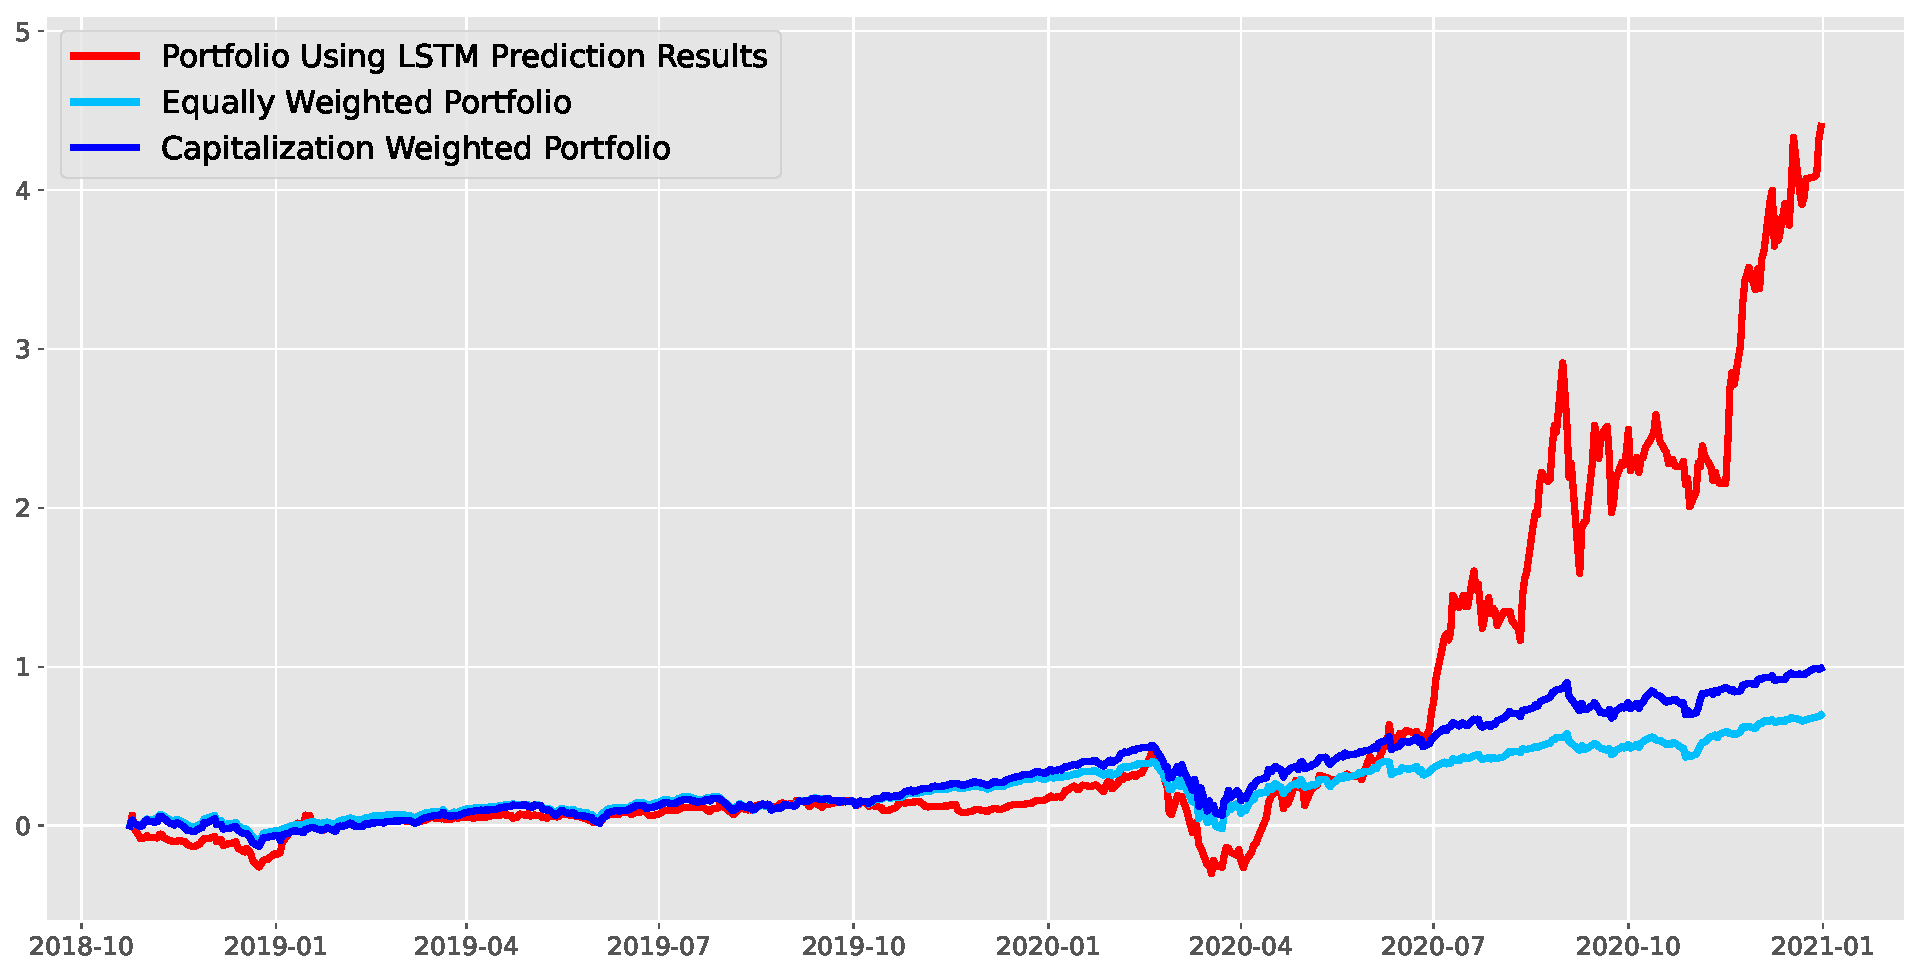
\includegraphics[width=0.9\textwidth]{images/portfolio_lstm.pdf}
    \caption{Portfolios performances in cumulative returns over time}
    \label{fig:portfolio_fin}
\end{figure}

\section{Comparison to other algorithms and datasets}
In this section, we show how to improve the algorithm and use different datasets and AI algorithms.

\subsection{Using Pytorch Lightning}
We revise the code by using Pytorch Lightning \cite{falcon2019pytorch}: this PyTorch framework provides a high-level interface by which it is easier to control architectures, results, logging and more. 
More importantly, it makes the process of moving models to GPU, Tensor Processing Units (TPUs) and even multiple GPUs and TPUs easier while having a negligible overhead. This open-source library is actively maintained by a community highly focused on efficiency and code readability. We refactor the code to be used with Pytorch Lightning.

\subsection{Results Comparison}
We show in Figure \ref{fig:portfolios_multi_same_dset} a comparison of the algorithms run with the same parameters with Pytorch Lightning and including RNN and GRU results and a version of LSTM with dropout.

\begin{figure}[h!]
    \centering
    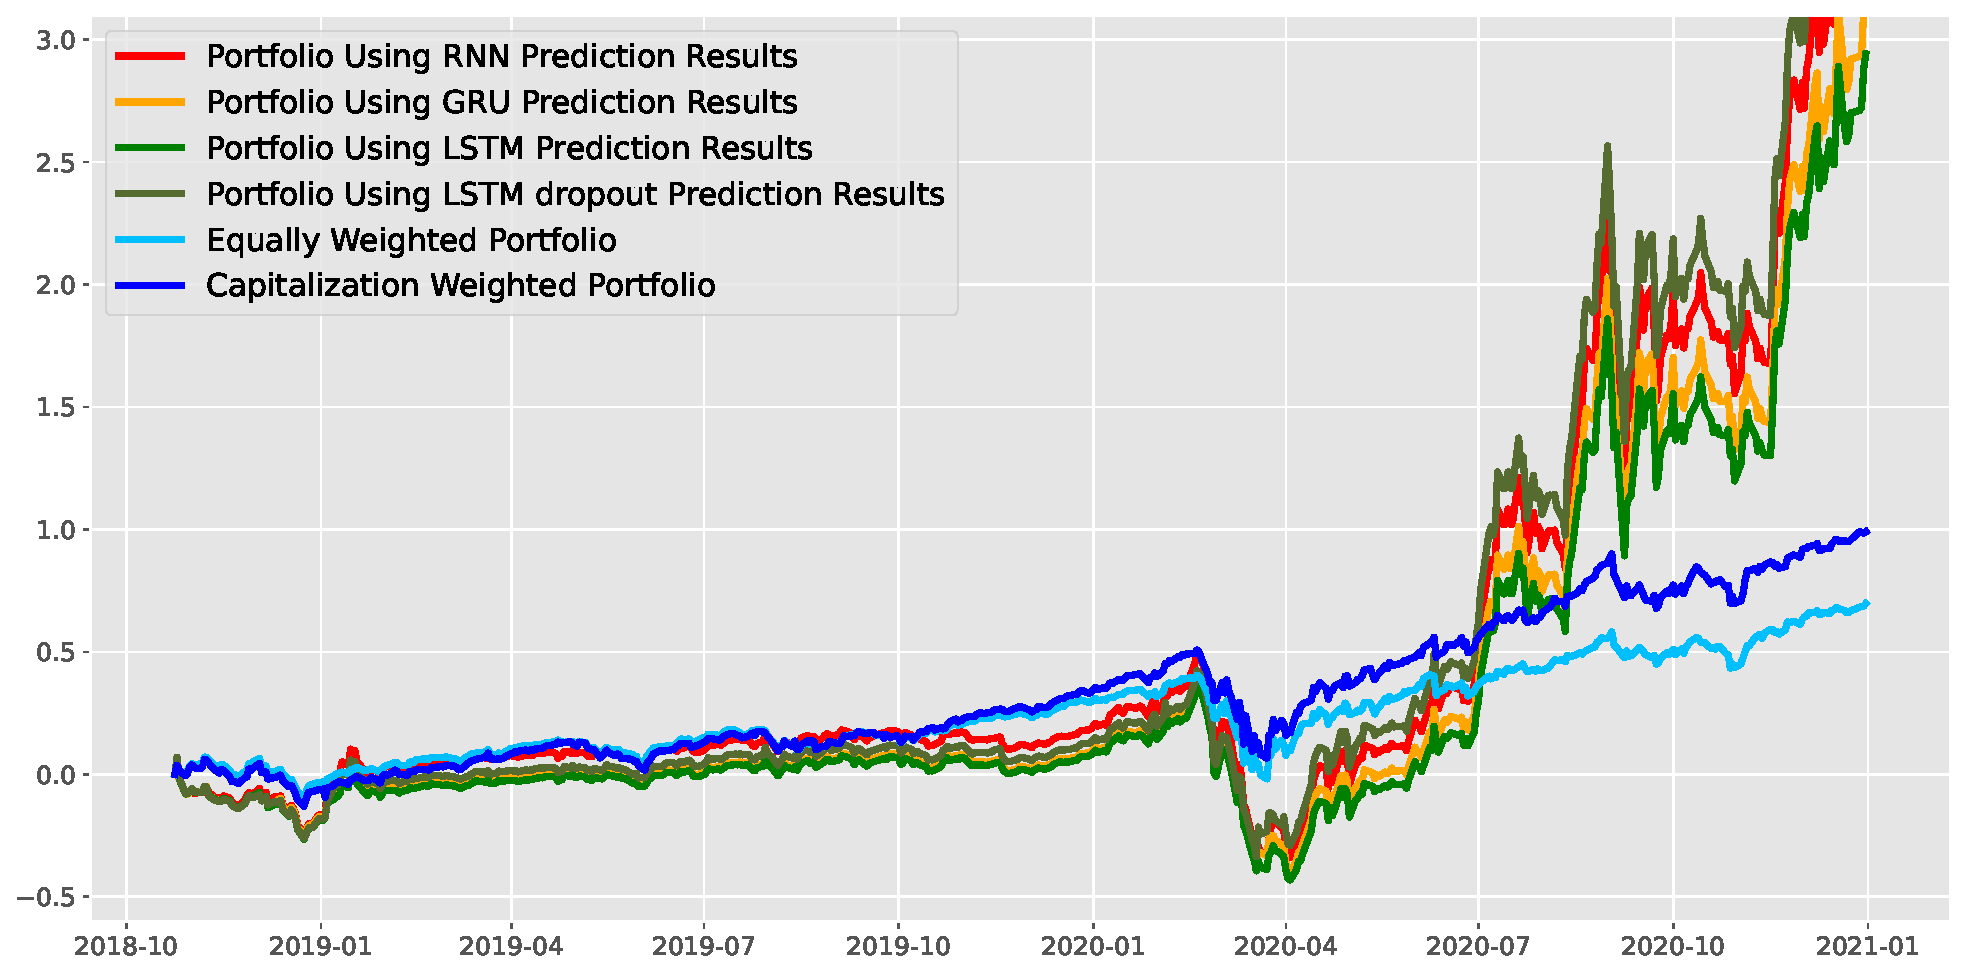
\includegraphics[width=0.9\textwidth]{images/portfolio_multi_same_dset.pdf}
    \caption{Portfolios performances in cumulative returns over time. As we can see, RNN and GRU perform similarly, while applying dropout as a regularization yields the best results.}
    \label{fig:portfolios_multi_same_dset}
\end{figure}

Moreover, we train on a new dataset: supposing we want to follow some online advice to invest in 10 stocks \footnote{Source: \href{https://money.usnews.com/investing/stock-market-news/slideshows/best-stocks-to-buy-this-year?slide=12}{US News Money}}. We can train our models and successfully get working portfolios with AI, which we show in Figure \ref{fig:portfolio_multi_new}

\begin{figure}[h!]
    \centering
    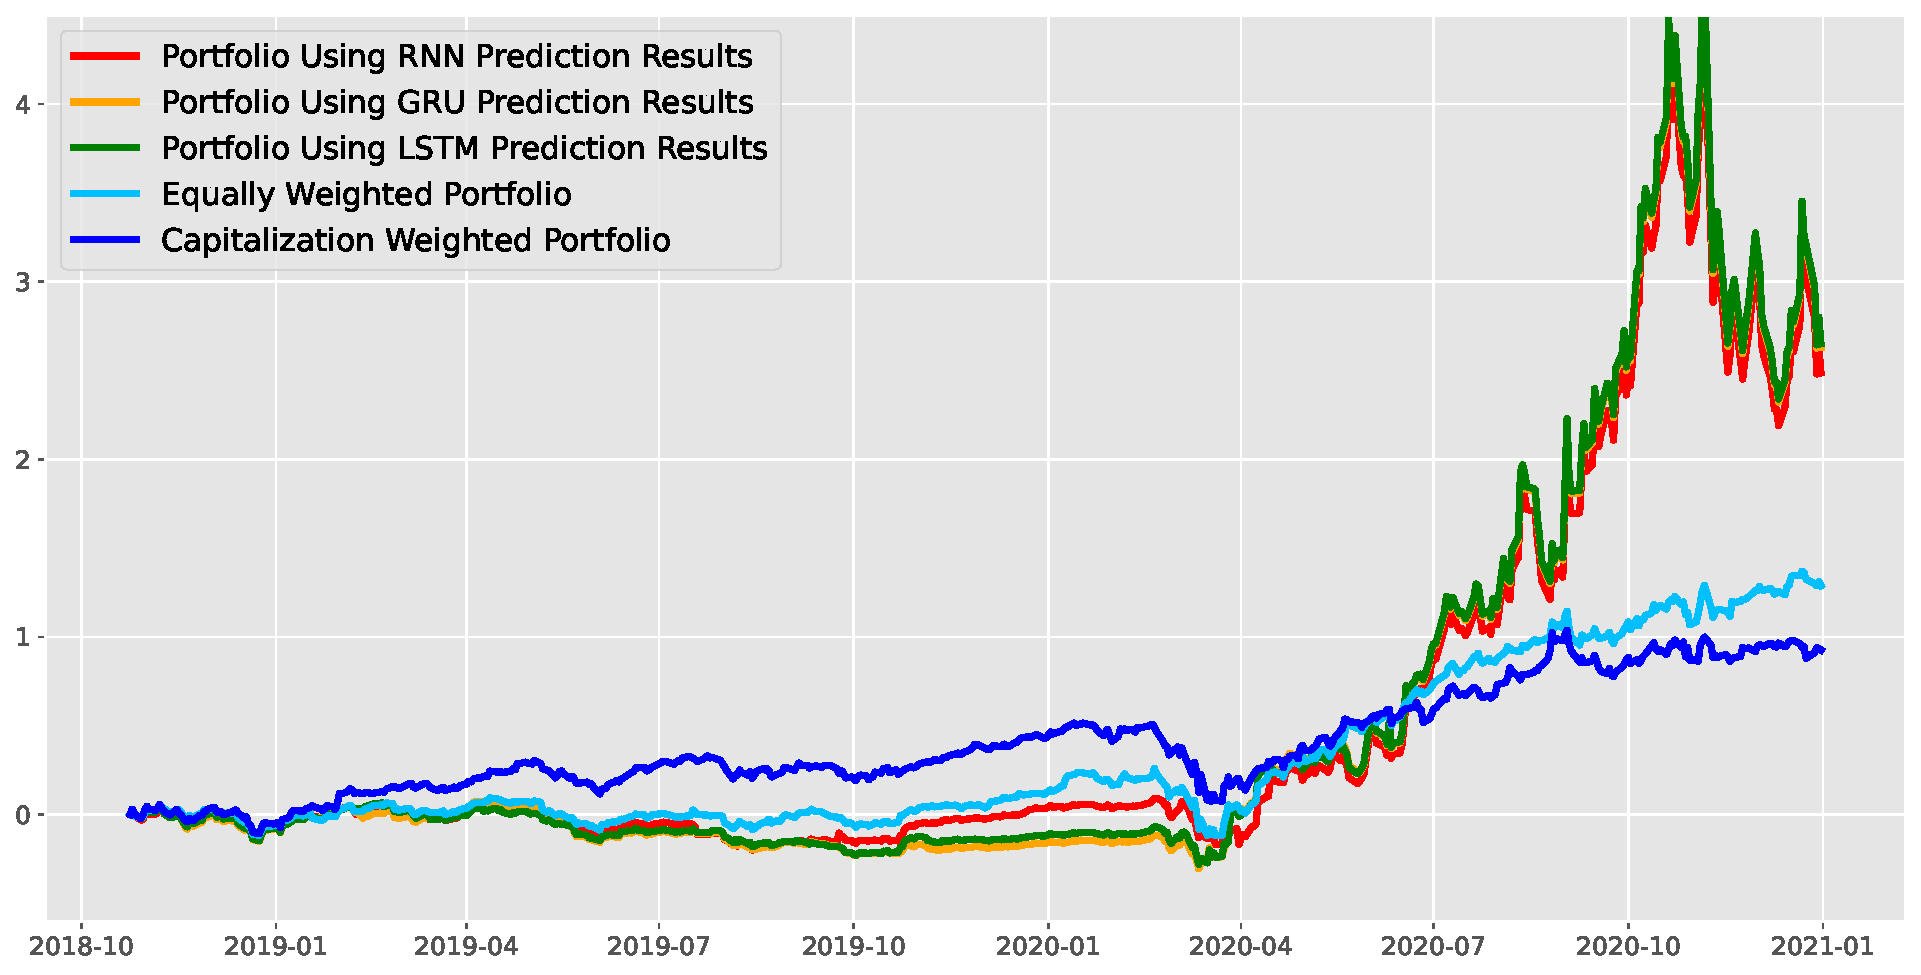
\includegraphics[width=0.9\textwidth]{images/portfolio_multi_new.pdf}
    \caption{Portfolios performances in cumulative returns over time. As we can see, RNN and GRU perform similarly to LSTM. Even though we may just have 10 stocks, the AI-driven portfolios are still able to outperform the Equally Weighted and the Capitalization Weighted ones.}
    \label{fig:portfolio_multi_new}
\end{figure}



 %%%%%%%%%% BIBLIOGRAPHY %%%%%%%%%% 
\bibliographystyle{plain}
\bibliography{ref}

\end{document}